\chapter{Methodology}


In this section, the data and the features are described. 
Subsequently, the model architecture is discussed and the explanation methods 
introduced in \cref{sec:xai} are framed in a chemical context. At last, 
the fidelity metric is introduced. The computational resources (Stevin Supercomputer 
Infrastructure) and services used in this work were provided by the VSC (Flemish 
Supercomputer Center), funded by Ghent University, FWO and the Flemish Government 
- department EWI.


\section{Data set description}


MoleculeNet provides publicly available benchmark data sets for the prediction of 
various molecular properties.\cite{wu2018moleculenet} Here, the ESOL data set is used,
which contains the measured solubility at $25^{\circ} C$ in $log(mol/L)$ for $1110$ 
distinct small molecules, each represented as a SMILES string.\cite{delaney2004esol}
From this representation various chemical properties can be computed using the RDKit python package\cite{landrum2010r}. 
The following properties are used to create the node feature vector: \cite{wu2023chemistry}

\begin{itemize}
    \item \textbf{Atom symbol:} One hot encoding of the atom type \\
        $\left( [B, C, N, O, F, Si, P, S, Cl, As, Se, Br, Te, I, At, metal] \right)$
    \item \textbf{Degree:} Number of covalent bonds (minimum is $0$ and maximum is $5$)
    \item \textbf{Formal charge:}\cite{parkin2006valence} The formal charge of an atom is defined as the difference between its valence 
        electrons and the number of electrons assigned from the Lewis structure where each single bond 
        contributes one electron. For example, nitrogen $(N)$ in nitrobenzene (\cref{fig:nitrobenzene})
        has a formal charge of $+1$, because $N$ has five valence electrons and gets four electrons 
        from the Lewis structure (one electron from each of the single bonds and two from the double bond).

        \begin{figure}[h]
            \centering
            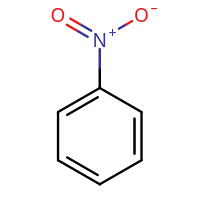
\includegraphics[scale=0.5]{nitrobenzene.png}
            \caption{Lewis structure of nitrobenzene}
            \label{fig:nitrobenzene}
        \end{figure}

    \item \textbf{Hybridization:}\cite{alabugin2015orbital} One hot encoding of the orbital structure of the atom \\
        $\left([sp, sp^2, sp^3, sp^3d, sp^3d^2, other]\right)$)

    \item \textbf{Aromaticity:} An aromatic system is a ring containing a delocalized electron 
        structure with $4n + 2$ electrons. For example, the benzene ring in \cref{fig:nitrobenzene}
        is an aromatic structure. ($0$ or $1$)

    \item \textbf{Hydrogens:} Hydrogen atoms are treated implicitly in order to prevent the
        explosion of the number of nodes in a molecular graph. If hydrogen atoms 
        were treated explicitly, then nitrobenzene (\cref{fig:nitrobenzene}) would 
        already have five more nodes, increasing the total nodes from ten to fifteen.
        (One hot encoding: $[0, 1, 2, 3, 4]$)

    \item \textbf{Chirality:}\cite{prelog1976chirality} Indicates whether the atom is a chiral center. Chirality 
        occurs when for example a carbon atom is bonded to four different groups. 
        Then the spatial orientation of those groups matters as not all configurations 
        are equivalent under rotation. ($0$ or $1$)

    \item \textbf{Chirality type:} One hot encoding of the chirality type $([R, S])$.

\end{itemize}


The type of an edge is determined by a bond feature vector consisting of the following chemical properties:


\begin{itemize}
    \item \textbf{Bond type:} One hot encoding of bond type ([single, double, triple, aromatic])
    \item \textbf{Conjugation:} Indicates whether the bond is part of a delocalized electron strucure.
        ($0$ or $1$) 
    \item \textbf{Ring:} Indicates whether the bond is part of a ring ($0$ or $1$).
    \item \textbf{Stereo:} One hot encoding of stereo configuration of the bond.
        ([StereoNone, StereoAny, StereoZ, StereoE])
\end{itemize}


\section{Architecture of the graph neural network model to predict water solubility}


Prediction of water solubility is achieved using the same RGCN model as Wu et. al. (\cref{fig:ml_model}),
with the hyperparameters listed in \cref{tab:hyperparameters}. To obtain more 
robust predictions, ten models are trained, each with a different seed 
$(2023 + 10i, \text{ with } i \in \{1, 2, \dots, 10\})$, where the final 
prediction is then obtained by the average prediction over all models.\cite{wu2023chemistry} 
The model is implemented in python using PyTorch Geometric\cite{Fey/Lenssen/2019}, training progress 
is tracked using wandb\cite{wandb} and analysis of the results is done using 
pandas\cite{reback2020pandas} an plotly\cite{plotly}.


\begin{figure}[h]
    \centering
    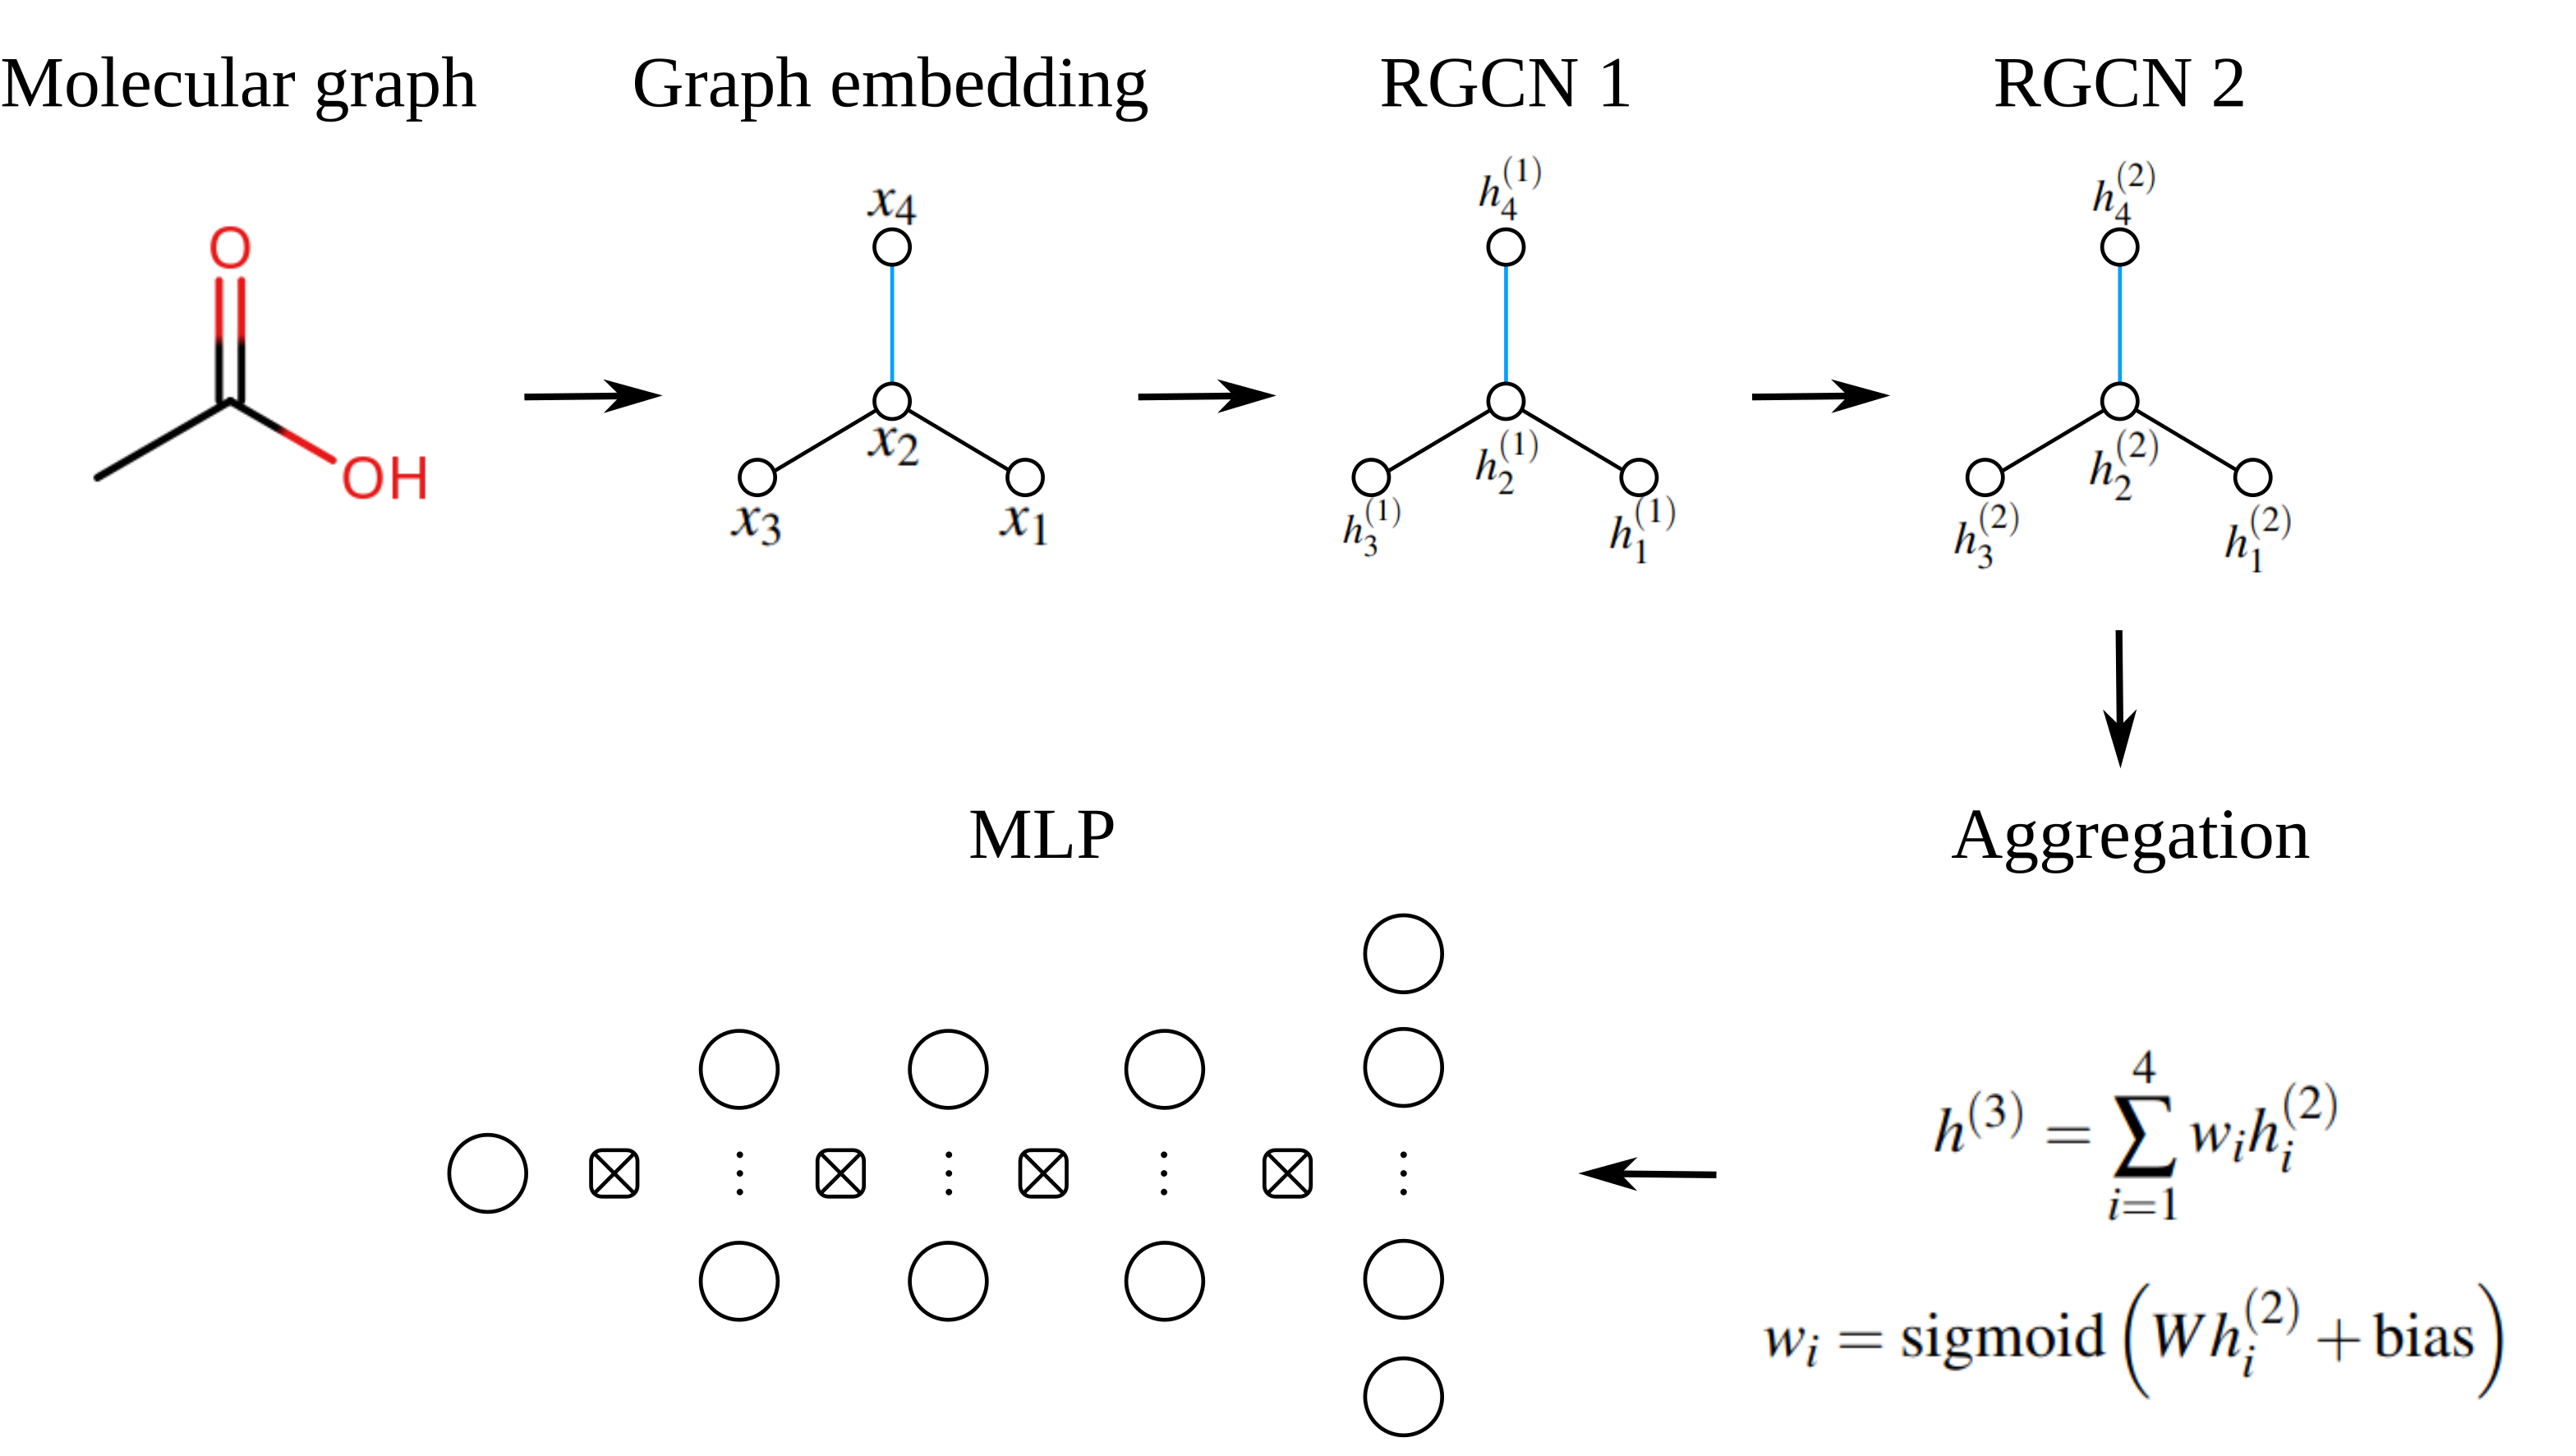
\includegraphics[scale=0.85]{rgcn_model.png}
    \caption{Machine learning model used for the prediction of water solubility of 
        small molecules. First, the molecular graph is embedded to a graph where the 
        bond features are used to determine edge types and node features are computed 
        using the RDKit python package. Next, two RGCN layers are applied, which are 
        followed by a weighted sum to aggregate the whole graph into one vector. This 
        vector is then passed to an MLP to obtain the final prediction.
    }
    \label{fig:ml_model}
\end{figure}


\begin{table}[h]
    \caption{ Hyperparameters from \protect\citen{wu2023chemistry} of an RGCN model to predict water solubility.}
    \label{tab:hyperparameters}
    \begin{center}
        \begin{tabular}{cc}
            \toprule
            \textbf{hyper parameter} & \textbf{value} \\
            \midrule
            RGCN layers & 2 \\
            RGCN hidden units & 256 \\
            RGCN dropout rate (each layer) & 0.5 \\
            MLP hidden units & 64 \\
            MLP dropout rate (each layer) & 0.1 \\ 
            Epochs & 500 \\
            Early stop & 30 \\
            \bottomrule
        \end{tabular}
    \end{center}
\end{table}


\newpage

\section{Chemically intuitive explanation}


In correspondence with the method developed by Wu et. al., a chemically intuitive 
explanation is obtain by first splitting a molecule into substructures.\cite{wu2023chemistry}
Two different substructure methods are used: functional groups and Breaking Retrosynthetically 
Interesting Chemical Substructures (BRICS). Functional groups are a collection of atoms 
having characteristic properties. Identification of functional groups within a molecule 
is achieved using SMILES Arbitrary Target Specification (SMARTS), which is a regular 
expression-like framework to match substructures in molecules.\cite{smartsDaylight}
Typically, a molecule is not just a combination of different functional groups. The 
remaining structure where all functional groups are attached to is referred to as the 
scaffold of the molecule (\cref{fig:example_functional_groups}). \Cref{app:functional_groups_list} 
lists the functional groups used in this study together with their corresponding SMARTS
representation. 


\begin{figure}[ht]
    \centering
    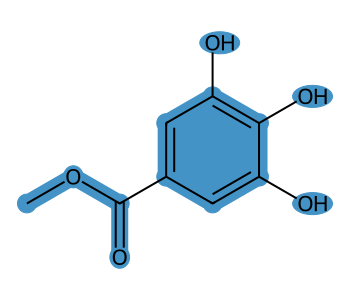
\includegraphics[scale=0.45]{../../data/images/example_functional_groups.png}
    \caption{An example of a molecule where the highlighted parts denote the different substructures. 
    The central benzene ring can be seen as the scaffold and the remaining four substructures are 
functional groups.}
    \label{fig:example_functional_groups}
\end{figure}


Some molecules do not posses any of the functional groups listed in \cref{app:functional_groups_list}. 
To explain these molecules, a BRICS\cite{degen2008art} partitioning scheme is used. BRICS breaks a molecule into possible 
chemical building blocks that could be used in a chemical reaction to synthesize the original 
molecule (\cref{fig:example_brices}).


\begin{figure}[h]
    \centering
    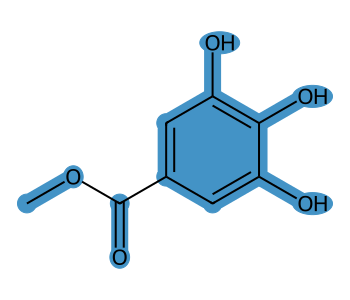
\includegraphics[scale=0.45]{example_brics}
    \caption{An example of a molecule where the highlighted parts are substructures obtained using BRICS.}
    \label{fig:example_brices}
\end{figure}

When the substructures of a molecule are obtained, the Shapley values and the HN values are 
computed. Within the game theoretical framework, a player represents a substructure and the 
characteristic function $v(S)$ is given by the difference between the model prediction $f(S)$ and 
the expected model prediction $\mathbb{E}[f(G)]$ over a random molecular graph $G$, which 
is estimated by the sample mean of the training data predictions,


\begin{equation}
    v(S) = f(S) - \mathbb{E}[f(G)].
\end{equation}


Since a substructure is a collection of atoms, a coalition of substructures is represented 
as a Boolean vector where a one indicates that the corresponding atom is part of a substructure 
included in the coalition and zero means that the atom is not included. This vector 
is then used in the aggregation step to only pass the information about the atom feature 
vectors $h_i^{(2)}$ that are present in the coalition to the MLP,


\begin{equation}
    h^{(3)} = \sum_{i=1}^N w_i h_i^{(2)} S_i,
\end{equation}

where $N$ is the number of atoms in the molecule.
Since the different attributions are compared using Spearman rank correlation, the
results are more meaningful when more than two substructures are present to obtain a non binary 
outcome. Therefore, the substructure method used for a molecule is the one that results 
in the most substructures. Only in \cref{sec:results_different_explanations} will we exclusive 
use functional groups. The full pipeline of the prediction and explanation 
of water solubility is shown in \cref{fig:pipeline}.


\begin{figure}
    \centering 
    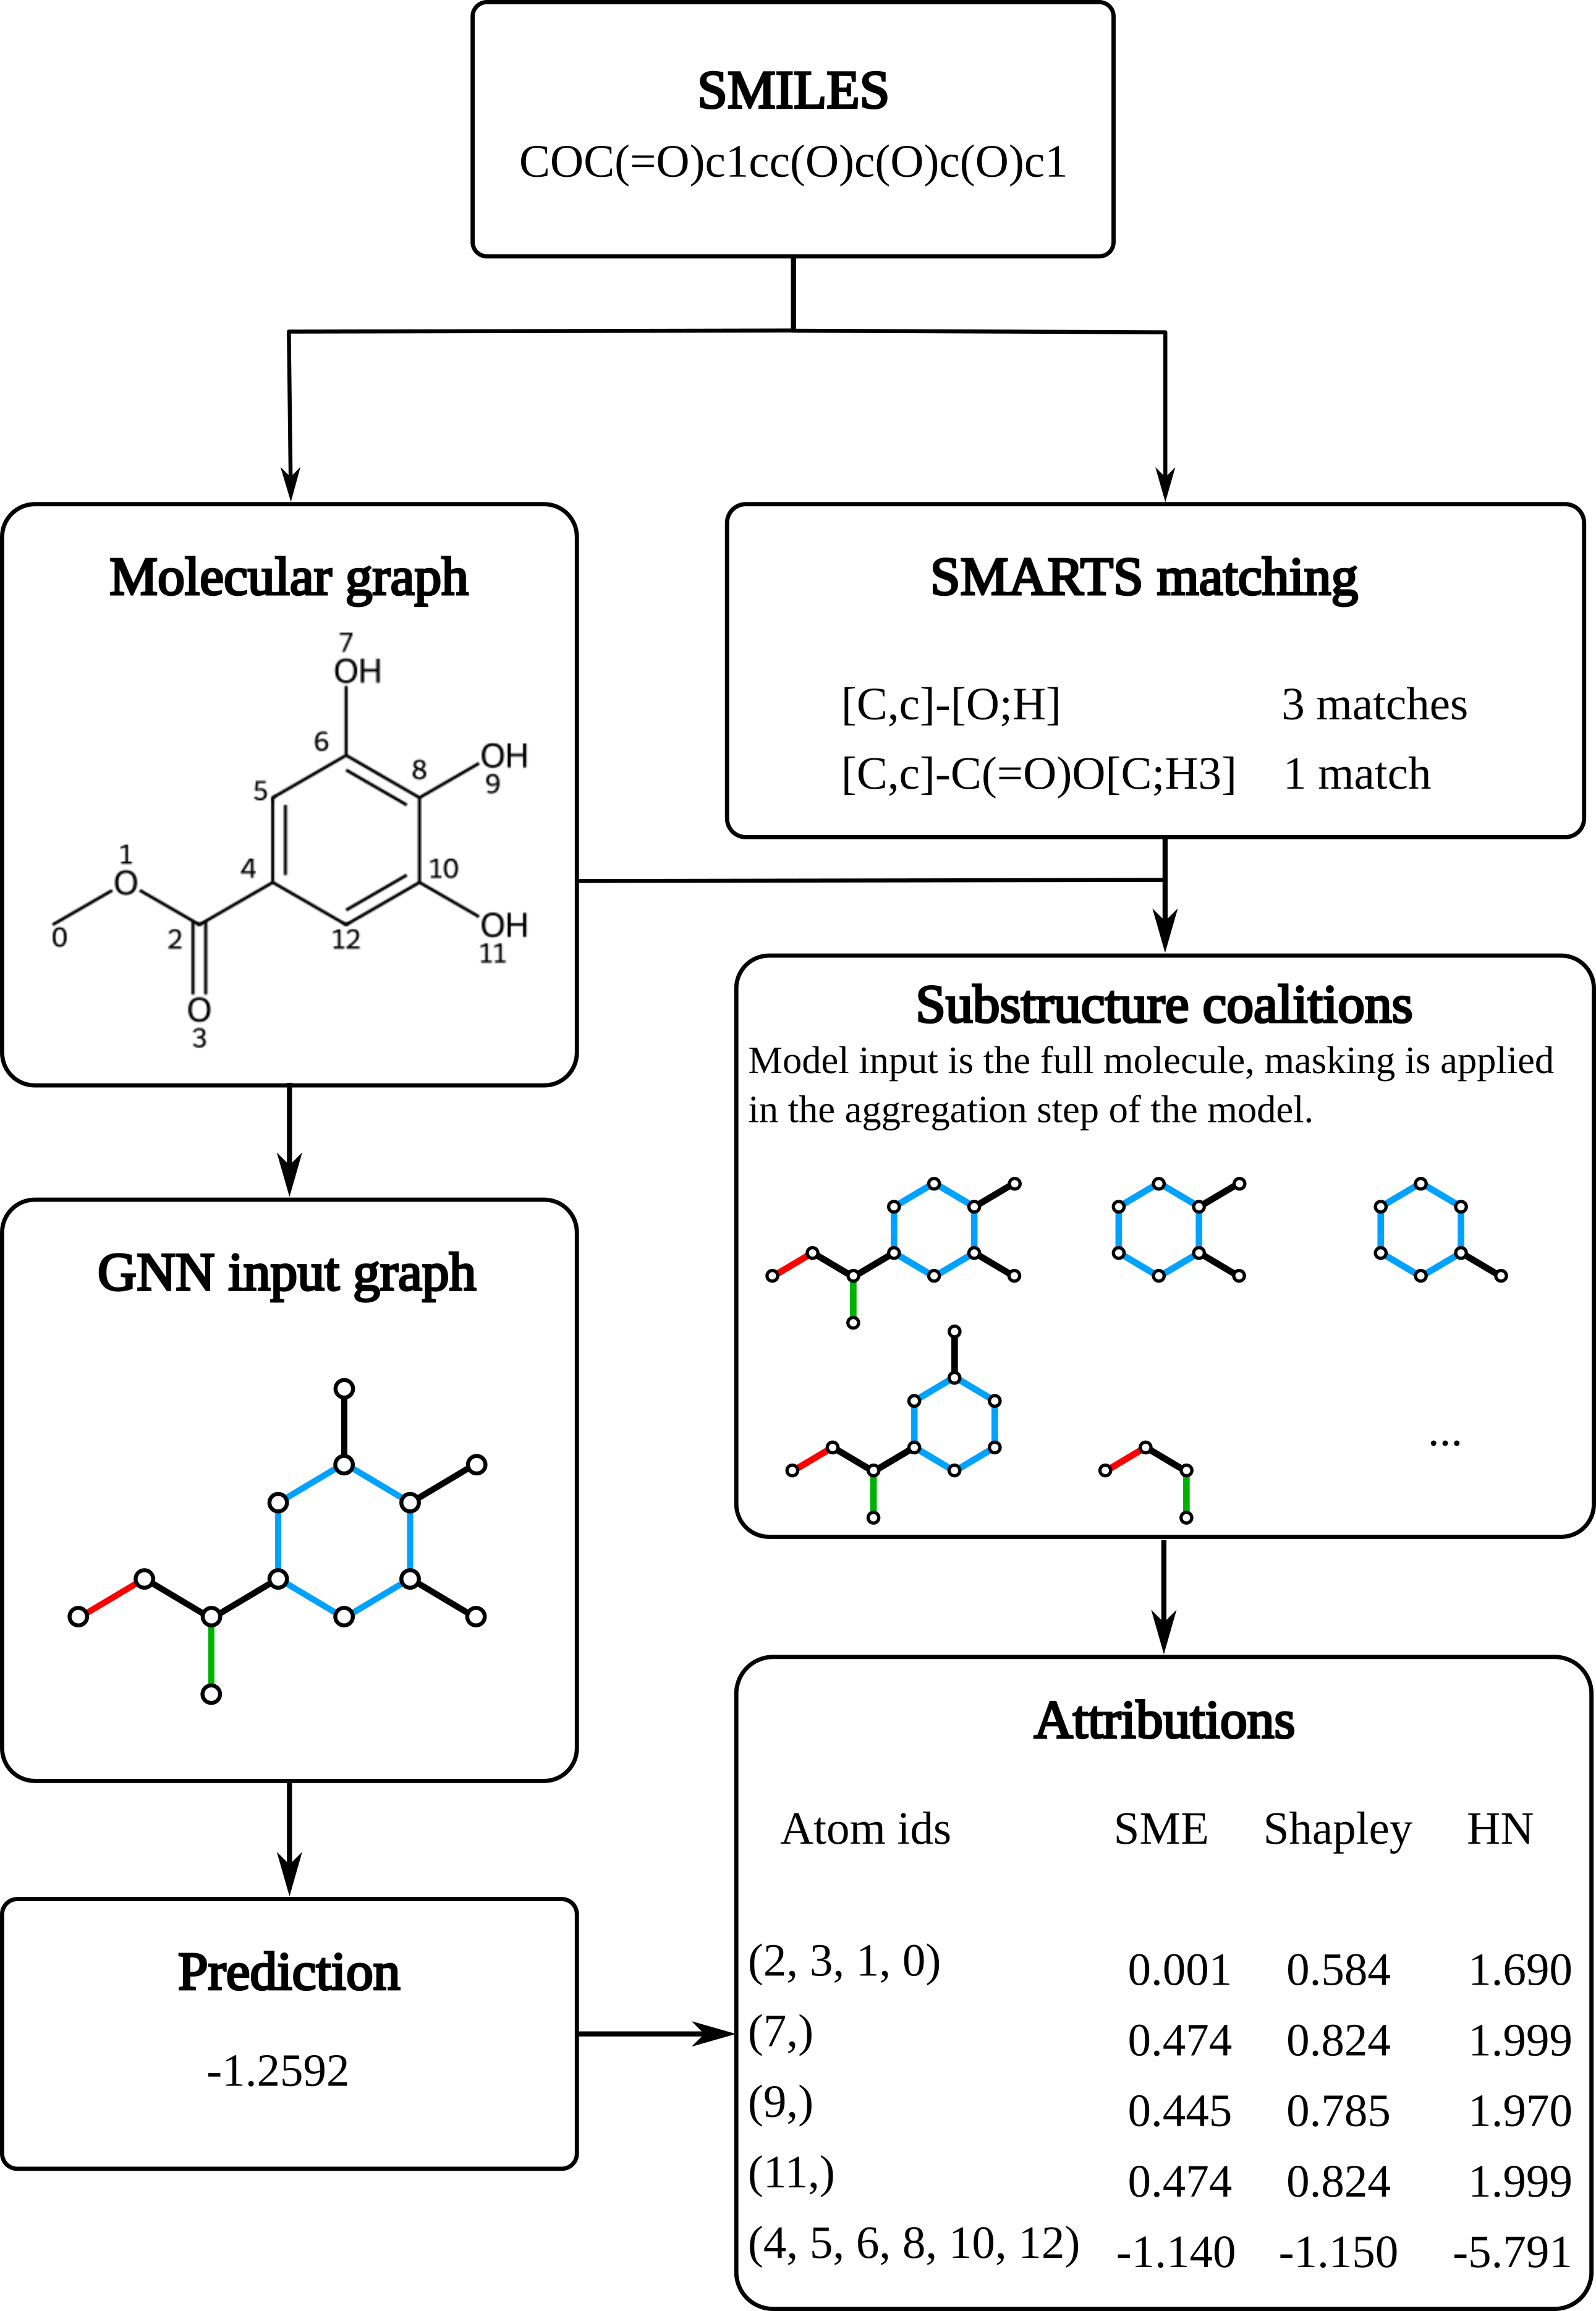
\includegraphics[scale=0.85]{explanation_pipeline}
    \caption{Pipeline to predict water solubility and explain the obtained prediction by means 
        of different attribution values. From a SMILES string a molecular graph is created and 
        the molecule is split into different substructures (BRICS also uses SMARTS pattern matching).
        Subsequently, atom and bond feature matrices are constructed based on the molecular graph. The 
        bond features then determine the edge types of the model input graph (denoted by different colors).
        Next, the model is evaluated on every combination between the different substructures by applying
        a mask in the aggregation step. Finally, the different attribution values can be computed.
    }
    \label{fig:pipeline}
\end{figure}


Because water is a polar molecule, substructures that increase the overall polarity 
of a molecule, will also increase the water solubility and hence are expected to obtain 
a positive attribution. Furthermore, when a substructure has the ability to form hydrogen 
bonds, it should have a higher positive attribution than when no hydrogen bonds can be 
formed. On the other hand, apolar substructures such as large carbon chains and polycyclic
compounds reduce the effect of smaller polar groups, resulting in a reduced 
water solubility. Therefore, apolar substructures should have negative attributions. 


\section{Evaluation of attribution methods}


Objective evaluation of an explanation method is not straightforward due to lack
of the ground truth. While a rank-based approach can evaluate the relative performance of attribution methods among 
themselves and relative agreement with chemical expectations, it provides no information on how faithful the 
explanation method is to the model. Assessment of model faithfulness can be done using the 
fidelity metric, which is a perturbation-based evaluation technique.\cite{yuan2022explainability} 
Fidelity assumes that removing an important feature (i.e. a feature with a high absolute attribution) will 
drastically change the model prediction. In contrast, features with an attribution around zero 
would not have a major impact on the model prediction.


Here, the removal of the most negative attribution (most hydrophobic) should result 
in a higher prediction. Since the difference between the original prediction and 
the perturbed prediction is expected to be negative, the removal of the most negative 
attribution is referred to as negative-fidelity. On the other hand, removing the most 
positive attribution (most hydrophilic) should result in a lower prediction, leading to a positive fidelity 
value, hence referred to as positive-fidelity. The fidelity corresponding with the removal 
of substructures that have an attribution around zero is referred to as low-absolute-fidelity.
